\section{An attack against PoPoW \cite{KLS}}
\label{sec:attack}

In this section, we revisit the construction for interactive proofs of
proof-of-work (PoPoW) from \cite{KLS} and its security.
PoPoW serves as the starting point and inspiration for our protocol.
%Their construction is also the
%starting point for our non-interactive PoPoW. We show that their construction is
However, the prior security proof is incorrect, and in fact the PoPoW protocol is susceptible to a double-spending attack within the model (i.e., that can be carried out by an attacker with less than 50\% hash power).
%they are susceptible to a double-spending attack even in the case the adversary controls
%a minority of the hashing power.

We proceed in two steps. We first show that a powerful attacker can break chain
superquality with non-negligible probability. Then we construct a concrete
double spending  attack based on this observation. Note that maintaining   chain
superquality was  not in the original security model; however, we show how the
property affects the security of the underlying blockchain proofs. %Our  concrete
%attack works under the assumption that the adversary has sufficient hashing
%power, but still below $50\%$.

%\subsection{The interactive proofs of proof-of-work protocol}
\paragraph{Interactive proofs of proof-of-work.}
In PoPoW, The main algorithm of the
verifier aims at distinguishing between two candidate proofs $(\pi_A, \chi_A)$
and $(\pi_B, \chi_B)$. The honest prover, having adopted $\chain_B$ during
mining, initially produces the proof $(\pi_B, \chi_B)$ as follows. First, the
last $k$ blocks are sent as $\chi_B = \chain_B[-k:]$. Then for the
first part of the chain, $\chain_B[:-k]$, the prover sets $\pi_B$ to be the
$\mu$-superchain spanning $\chain_B$ for the largest $\mu$ such that $|\pi_B| =
m$, where $m$ is the protocol's security parameter. The verifier ensures that
$|\pi_A| \geq m, |\pi_B| \geq m$ so that the proofs are not shorter than $m$ and
then checks whether $\pi_A = \pi_B$; if so, the decision is drawn immediately
based on $\chi_A,\chi_B$ without interaction. Otherwise, the verifier queries
the provers for their claimed anchored superchains $\chain_A\upchain^\mu$,
$\chain_B\upchain^\mu$ at some level $\mu$. The verifier starts querying at the
highest possible level $\mu$ and descends until level $\mu$ is sufficiently low
such that $b = LCA(\pi_A\upchain^\mu, \pi_B\upchain^\mu)$ is $m$ blocks from the
tip of the chain for one of the proofs. That is, the querying stops at such
$\mu$ when $max(|\pi_A\upchain^\mu\{b:\}|, |\pi_B\upchain^\mu\{b:\}|) \geq m$.
The winner is designated as the prover with the most blocks after $b$ at that
level; i.e., $A$, if $|\pi_A\upchain^\mu\{b:\}| \geq |\pi_B\upchain^\mu\{b:\}|$,
and $B$ otherwise. The communication overhead is reduced by only requesting
blocks after the purported LCA. The security parameter $m$ is chosen to ensure
%application of a binomial Chernoff bound:
that the probability of the attacker
producing a long superchain is negligible.

%\subsection{Attacking chain superquality}
\paragraph{Attacking chain superquality.}
\label{subsec.superquality-attack}
We construct an adversary $\mathcal{A}$ that breaks the superchain quality at level $\mu$.
% Suppose $\mathcal{A}$ controls a portion $t/n$ of the hashing power.
$\mathcal{A}$ works as follows. Assume she wants to attack the honest party $B$
in order to have him adopt chain $\chain_B$ which has a bad distribution of
superblocks, i.e. such that local goodness is violated in some sufficiently long
subchain. She continuously determines the current chain $\chain_B$ adopted by
$B$. The adversary starts playing after $|\chain_B| \geq 2$. If
$\textit{level}(\chain_B[-1]) < \mu$, then $\mathcal{A}$ remains idle. However,
if $\textit{level}(\chain_B[-1]) \geq \mu$, then $\mathcal{A}$ attempts to mine
an adversarial block $b$ on top of $\chain_B[-2]$. If successful,  she attempts
to mine another block $b'$ on top of $b$. If successful again, she broadcasts
$b$ and $b'$. The adversarial mining continues until $B$ adopts a new chain,
which can be due to two reasons: Either the adversary successfully mined $b, b'$
on top of $\chain_B[-2]$ and $B$ adopts them; or one of the honest parties mined
a block which was adopted by $B$. In either case, the adversary restarts
the strategy by inspecting $\chain[-1]$ and acting accordingly. An execution of
this attack is illustrated in Figure~\ref{fig.superquality-attack}.

\begin{figure}
    \caption{Superquality attack on prior work (PoPoW)~\cite{KLS}.
    The adversary performs a selfish-mining~\cite{selfish} attack (gray blocks)
    whenever any honest parties have recently mined a rare $\mu$-superblock (black). The attack reduces the honest chain's superquality, while the attacker's private chain is unaffected. }
    \centering
    \iftwocolumn
        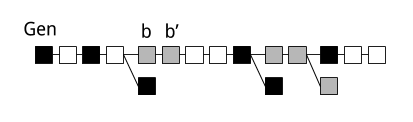
\includegraphics[width=\columnwidth,keepaspectratio]{figures/superquality-attack-popow.png}
    \else
        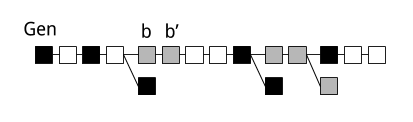
\includegraphics[width=0.5 \columnwidth,keepaspectratio]{figures/superquality-attack-popow.png}
    \fi
    \label{fig.superquality-attack}
\end{figure}

Assume now that an honestly-generated $\mu$-superblock was adopted by $B$ at
position $\chain_B[i]$ at round $r$. We now examine the probability that
$\chain_B[i]$ will remain a $\mu$-superblock in the long run. Suppose $r' > r$
is the first round after $r$ during which a block is generated. $\mathcal{A}$
will succeed in this attack with non-negligible probability and cause $B$ to
abandon the $\mu$-superblock from their adopted chain. Therefore, there
exists $\delta$ such that the adversary will be able to cause $\delta$-variance
with non-negligible probability in $m$. This suffices to show that superquality
is violated.

As seen in the illustration, while the honest parties have generated several
$\mu$-superblocks, some of them are in blockchain forks which have been
abandoned, causing a superquality harm.

\paragraph{A double-spending attack.}
Extending the above attack, we modify the superquality attacker into an attacker
that causes a double spending attack in the PoPoW construction. We first give
a sketch of the attack.

As before, $\mathcal{A}$ targets the proofs generated by honest party $B$ by
violating $\mu$-superquality in $B$'s adopted chain. $\mathcal{A}$ begins by
remaining idle until a certain chosen block $b$. After block $b$ is produced,
$\mathcal{A}$ starts mining a secret chain which forks off from $b$ akin to a
selfish mining attacker~\cite{selfish}. The adversary performs a normal spending
transaction on the honestly adopted blockchain and has it confirmed in the block
immediately following block $b$. She also produces a double spending transaction
which she secretly confirms in her secret chain in the block immediately
following $b$.

$\mathcal{A}$ keeps extending her own secret chain as usual. However, whenever a
$\mu$-superblock is adopted by $B$, she temporarily pauses mining in her secret
chain and devotes her mining power to harm the $\mu$-superquality of $B$'s
adopted chain. Intuitively, for large enough $\mu$, the time spent trying to
harm superquality will be limited, because the probability of a $\mu$-superblock
occurring will be small. Therefore, the adversary's superchain quality will be
larger than the honest parties' superchain quality (which will be harmed by the
adversary) and therefore, even though the adversary's $0$-chain will be shorter
than the honest parties' $0$-chain, the adversary's $\mu$-superchain will be
longer than the honest parties' $\mu$-superchain and thus will be favored by the
verifier! The formal calculation of the probability of this attack succeeding is
in the next section. We note that  actually, for appropriate choice of system
parameters, the attack can be made to succeed with overwhelming probability.
A concrete parameterization of the attack is given in the
% \iftr
% \else
full online version.
% \fi

% AM: suppressed for anonymization
%\footnote{We wish to thank Giorgos Panagiotakos, Peter Ga\u{z}i, and Nikos
%Leonardos for their insights.}

